% !TeX root = ../main.tex

\chapter{緒論}

本章為緒論,將簡述國內外電力需求狀況與傳統發電之困境,並分別從電力系統發展、再生能源發展、電動汽車發展與我國能源政策面相切入研究背景,最後說明本研究預期達到的目標以及章節組成架構。

\section{前言}

能源是人類社會維持生存與文明發展所不可或缺的基礎,但隨著經濟發展與科技進步所延伸出的能源危機、空氣汙染與溫室效應,儼然已是世界各國不得不面對的緊迫難題。

% 電力需求持續成長
長期以來,國內外的電力需求持續成長,圖 \ref{figure: Yearly Electricity Consumption in Taiwan} 的臺灣地區年度用電數量 \cite{boe-data} 顯示自 $1999$ 年至 $2018$ 年間,臺灣地區的年度用電數量由 $1,609$ 億度($160.9$ \si{\TWh})成長至 $2,665$ 億度($266.5$ \si{\TWh});於此同時,圖 \ref{figure: Yearly Electricity Consumption over World} 的世界各國年度用電數量 \cite{enerdata-ec} 亦顯示世界各國的年度用電量由 $126,120$ 億度($12612$ \si{\TWh})成長至 $229,640$ 億度($22964$ \si{\TWh}),其中又以我國在內的亞洲地區成長最為顯著。考量未來產業變遷、電動汽車普及…等新增用電需求,我國經濟部推估至 $2025$ 年間,臺灣地區用電數量每年將成長約 $1.86\%$,年度用電量將達到 $3,029$ 億度($302.9$ \si{\TWh}) \cite{boe-107report}。

% 年度用電量統計數據
\begin{figure}[hbp]
  \centering
  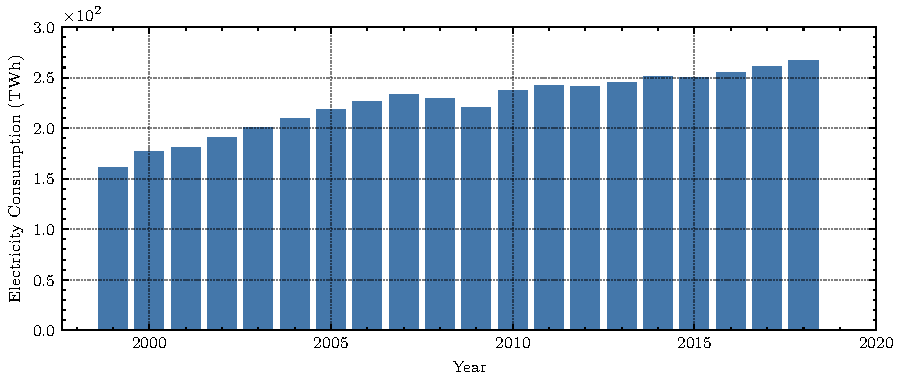
\includegraphics[width=\textwidth]{Yearly Electricity Consumption in Taiwan}
  \caption[臺灣地區年度用電量]{臺灣地區年度用電數量 \cite{boe-data}}
  \label{figure: Yearly Electricity Consumption in Taiwan}
  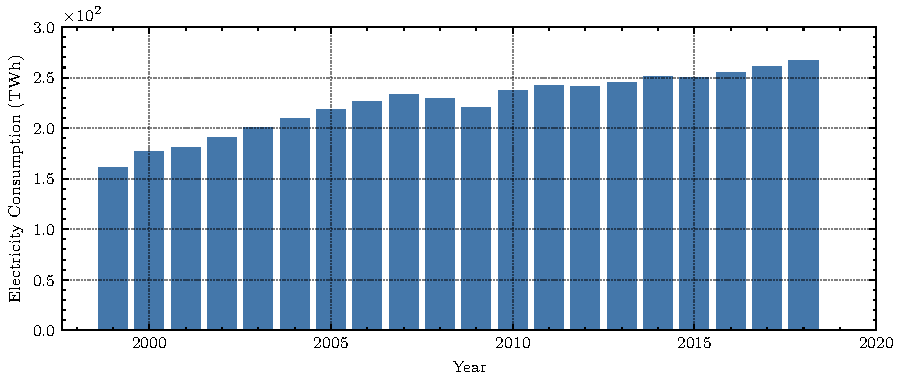
\includegraphics[width=\textwidth]{Yearly Electricity Consumption in Taiwan}
  \caption[世界各地年度用電量]{世界各地年度用電數量 \cite{enerdata-ec}}
  \label{figure: Yearly Electricity Consumption over World}
\end{figure}

% 傳統發電佔比與缺點
目前世界各國的電力來源主要以火力發電與核能發電為主,根據統計,在 $2018$ 年時,火力發電與核能發電約佔臺灣地區總發電數量的 $94.19\%$ \cite{boe-data},火力發電與核能發電約佔全球總發電數量的 $74\%$ \cite{iea-wegs}。其中火力發電需要大量開發燃煤、石油與天然氣…等不可再生能源,同時也導致相關產業的溫室氣體排放量居高不下;而核能發電有著較高的發電效率,並且幾乎沒有空氣汙染問題,但隱含安全隱憂,比如 $1986$ 年發生於俄羅斯的\uline{車諾比}事件(Chernobyl disaster)、$1979$ 年發生於美國的\uline{三哩島}事件(Three Mile Island accident)與 $2011$ 年發生於日本的\uline{福島}第一核電廠事故(Fukushima Daiichi nuclear disaster)。

在民眾環保意識抬頭與核能發電安全隱憂的時空背景下,世界各國開始重新審視既有的能源產業與政策。於此同時,能夠充分利用再生能源,具有良好的環境效益的分散式發電(Distributed Generation, DG)技術近年來受到越來越多的關注,但礙於起初設計輸配電網路時並未納入考慮,為解決此問題,整合分散式能源(Distributed Energy Resources, DERs)、可控式負載與儲能設備(Battery Energy Storage, BESS)為一個整體,使其參與電力系統運行與電力市場交易的虛擬電廠(Virtual Power Plant, VPP)概念也應運而生。

\section{研究背景}

\subsection{電力系統發展}

% 電力系統定義
電力系統是指由發電系統、輸電系統與配電系統所組成的複雜系統,負責處理電力供給中所依序會經歷的發電、輸電、配電與用電四個過程 \cite{vignolo2001transmission}。目前包含臺灣本島、澎湖、金門與馬祖在內的中華民國地區電力供應,由隸屬於我國經濟部的國營事業機構──臺灣電力股份有限公司(簡稱台電)負責。如圖 \ref{figure: Taiwan Power System Structure} 所示,台電公司供電系統中核能、水力與火力發電廠產生電力後,需透過變壓器將電壓升至 $345$ 仟伏特($345$ \si{\kV}),再利用輸電線路輸送電力,最後透過高壓變電所與一次變電所分別降壓至 $161$ 仟伏特($161$ \si{\kV})、$69$ 仟伏特($69$ \si{\kV})後,提供給科學園區、工業園區及大眾運輸工具…等大型用戶用電,並透過配電變電所、二次變電所及配電系統再進行降壓,提供一般用戶做為民生用電使用。\cite{taipower-sps}

% 台電供電系統
\begin{figure}[htbp]
  \centering
  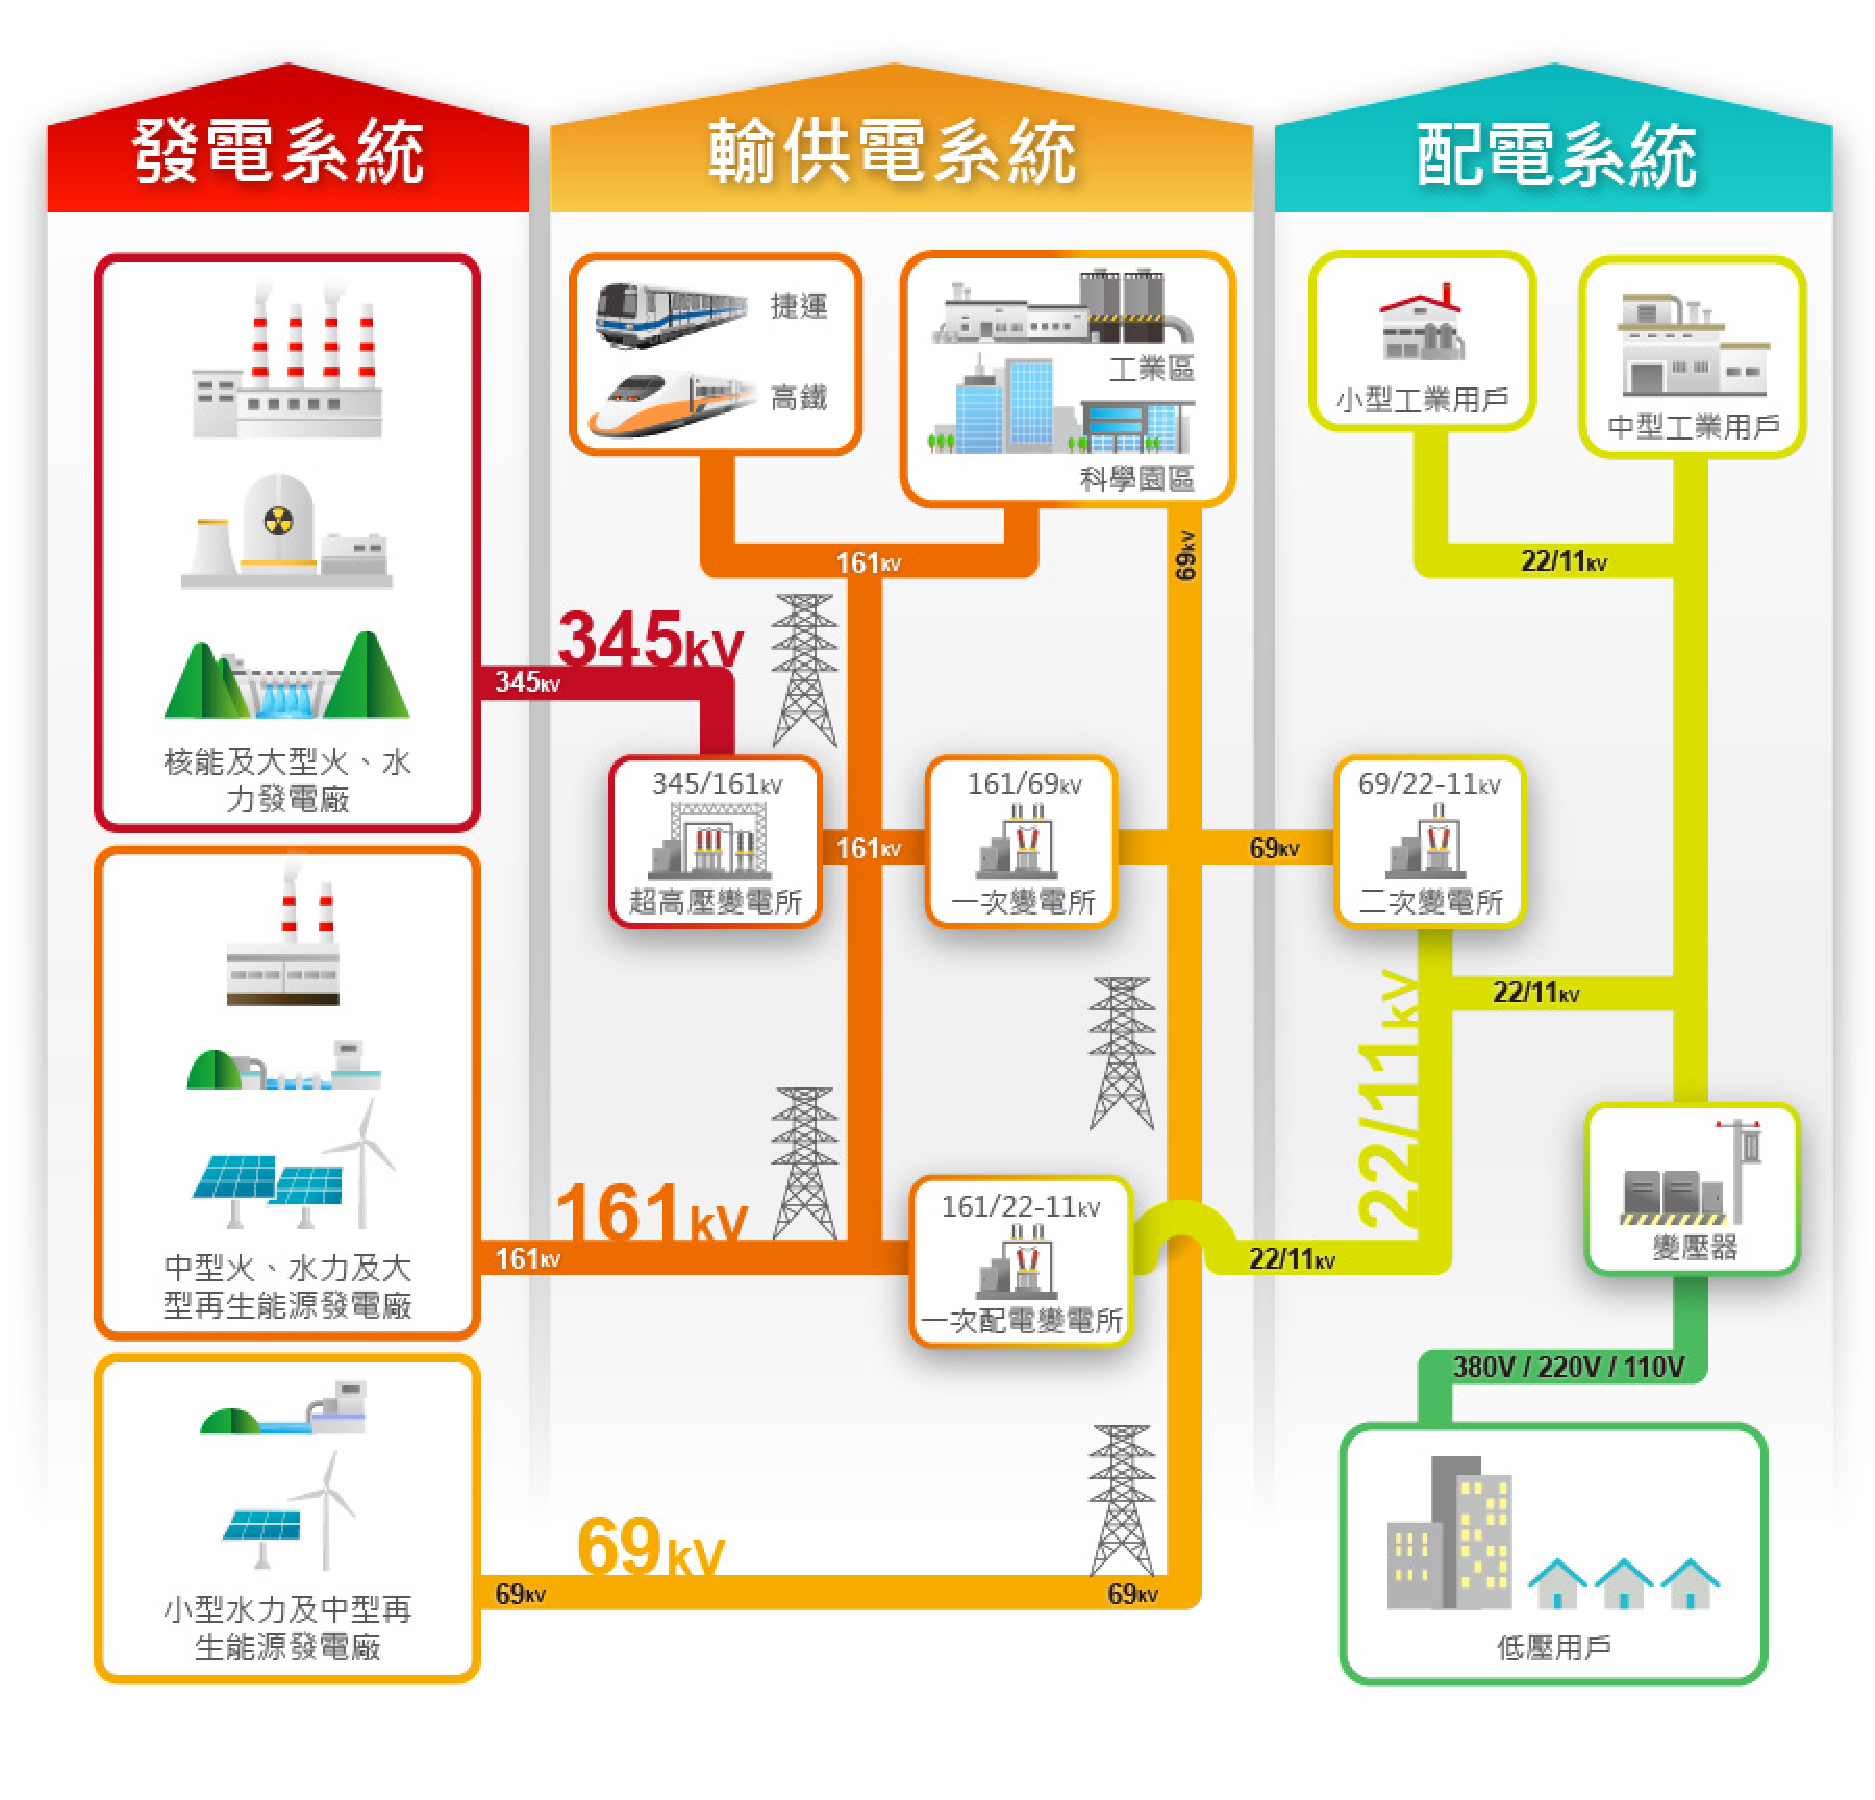
\includegraphics[width=0.75\textwidth]{Taiwan Power System Structure}
  \caption{臺灣電力公司供電系統}
  \label{figure: Taiwan Power System Structure}
\end{figure}

% 傳統電網問題
目前世界各國的電力系統仍以傳統集中式大型電網系統為主,雖然長期以來具有很好的規模經濟效益,然而隨著經濟與科技發展,人們對於能源供給穩定性的要求日益提高,傳統集中式大型電網系統的缺陷也逐漸浮現。傳統集中式大型電網系統所面臨的問題,大致上可以歸納為以下幾點:

\begin{itemize}
  \item \textbf{發電機組集中建設,長距傳輸能量折損}:考量建設成本,發電機組與用電用戶所在地通常距離遙遠,容易導致電力生產與分配不均,需要跨區輸電來解決電力不足問題,長距離的電力傳輸過程所累積的能量損失亦十分可觀。以臺灣地區為例,輸電系統分為北、中、南三個地區,過去資料顯示在用電尖峰季節,北部地區電力仍需中南部地區補足,過去十年間臺灣地區電力的線路損失率約為 $4\%$。\cite{boe-data}
  \item \textbf{局部故障影響整體,可靠穩定備受考驗}:傳統電網中,超過負載的高壓電纜將使得過載電流必須由附近的其他輸配電纜負責分攤,大量的電流回流可能導致輸配電纜超出負載而燒斷,故障擴散進而導致大面積的停電效應。比如 $2003$ 年美加大停電(影響人數達 $5,000$ 萬人)、$2006$ 歐洲大停電(影響人數達 $1,200$ 萬人)和 $2012$ 年印度大停電(影響人數達 $62,000$ 百萬人)…等大規模停電事件。
%   \item 無法靈活追蹤負荷變化
  \item \textbf{發電倚賴化石燃料,背離能源永續目標}:燃煤、石油與天然氣…等火力發電燃料屬於不可再生能源,生產電力過程中也伴隨著溫室氣體的排放,核能發電亦隱含安全隱憂。國際間越趨重視相關環境保護與資源永續問題,傳統集中式大型電網的主要發電方式勢必需要進行改善。
\end{itemize}

% 分散式發電、智慧電網、微電網
相對於傳統集中式大型電網系統,能夠充分利用再生能源的分散式發電(Distributed Generation, DG)技術近年來備受關注,國內外許多文獻對於分散式發電並沒有規範的定義,一般是指分散地布置於用電用戶周圍,容量較小的發電裝置 \cite{nissen2009high}。由於短時間內無法完全取代傳統集中式大型電網系統,目前的分散式電源多以接入既有電網運行為主,為了儘量減少併入分散式電源所引起的網路耗損與可靠性降低,世界各國均致力於發展智慧電網(smart grid)與微型電網(microgrid)技術。前者結合電力系統與資訊系統,利用資訊與通訊技術進行電力設備的自動化與最佳化;後者整合多個分散式電源組成拓譜結構,並可以自由切換連接模式或孤島模式,提升電力系統可靠度。

\subsection{再生能源發展}

為了抑制持續嚴峻的全球暖化現象,聯合國於 $1997$ 年簽署「\uline{京都}議定書」規範工業國家未來溫室氣體排放目標,因此各國逐漸將能源產業開發重心轉移至核能發電與再生能源發電。

表 \ref{table: Distributed Generation Emissions Data} 為常見分散式發電技術的主要污染物排放量 \cite{carter2000emissions},顯示再生能源普遍具有潔淨低環境汙染的特性,其中又以風力發電與太陽能發電在發電過程中不會排放汙染物表現最佳。除此之外,近年來更有研究表示風力發電與太陽能發電能夠緩解地下水水位下降,進一步降低供水壓力與糧食危機。\cite{He2019}

\begin{table}[htp]
  \centering
  \caption[常見分散式發電技術主要污染物排放量]{常見分散式發電技術主要污染物排放量 \cite{carter2000emissions}}
  \begin{tabular*}{\textwidth}{@{\extracolsep{\fill}}cccccc}
    \toprule
    \textbf{發電技術} & \textbf{\ce{CO2}} & \textbf{\ce{NOx}} & \textbf{\ce{SO2}} & \textbf{\ce{CO}} & \textbf{PM-10} \\
    \midrule
    內燃機組    & $444.52$ \~{} $498.95$ & $0.14$ \~{} $2.72$ & 可忽略 & $0.91$ \~{} $4.08$ & $0$ \~{} $0.27$ \\
    燃料電池    & $362.87$ \~{} $635.03$ & $< 0.02$ & $0$ & $0.01$ \~{} $0.05$ & 可忽略 \\
    生物質能    & $0$ \~{} $1043.26$ & $0.14$ \~{} $2.72$ & $< 0.14$ & $0.91$ \~{} $4.08$ & $0.27$ \~{} $1.81$ \\
    風力發電    & $0$ & $0$ & $0$ & $0$ & $0$ \\
    太陽能發電  & $0$ & $0$ & $0$ & $0$ & $0$ \\
    \bottomrule
    & & & & & \si[per-mode=symbol]{\kilogram\per{\mega\watt\cdot\hour}}
  \end{tabular*}
  \label{table: Distributed Generation Emissions Data}
\end{table}

根據歷年統計資料,全球的風力發電累計裝置容量從 $2000$ 年僅 $18,039$ 千瓩($18,039$ \si{\MW}),成長至 $2018$ 年的 $591,091$ 千瓩($591,091$ \si{\MW});全球的太陽能發電累計裝置容量則自
$2000$ 年僅 1,288 千瓩($1,288$ \si{\MW}),成長至 $2018$ 年的 $509,300$ 千瓩($509,300$ \si{\MW})。圖 \ref{figure: Global Wind and Solar Power Installation} 為 $1980$ 年至 $2019$ 年的全球風力發電與太陽能發電累積裝置容量 \cite{wei-data, statista-pv},顯示近年來不論是風力發電亦或是太陽能發電皆發展迅速。

% 風機裝置容量
\begin{figure}[htbp]
  \centering
  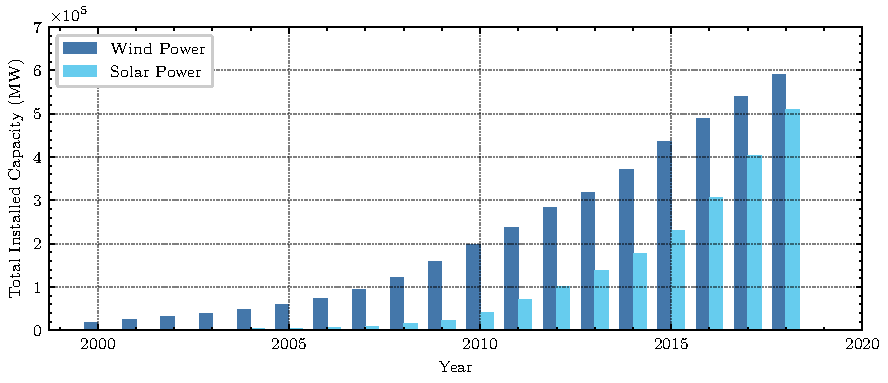
\includegraphics[width=\textwidth]{Global Wind and Solar Power Installation}
  \caption[全球風力發電與太陽能發電累積裝置容量]{全球風力發電與太陽能發電累積裝置容量 \cite{wei-data, statista-pv}}
  \label{figure: Global Wind and Solar Power Installation}
\end{figure}

受到招標、競標及綠色憑證等市場機制、世界各國政策政策支持與建置成本逐漸降低…等因素影響,風力發電與太陽能發電等再生能源發展前景十分強勁,全球風能協會(Global Wind Energy Council, GWEC)預估到 $2024$ 年風力發電將再有約 $300,000$ 千瓩($300,000$ \si{\MW})的新增裝置容量 \cite{ohlenforst2019global},國際能源署(International Energy Agency, IEA)則預估到 $2024$ 年時,太陽能發電的新增裝置容量將成長至 $600,000$ 千瓩($600,000$ \si{\MW}) \cite{iea2019report}。

\subsection{電動汽車發展}

隨著再生能源的發展,輸配電網對環境越趨友善的同時,也帶動了電動車產業的革新以及電力需求的成長。電動汽車(Electric Vehicle, EV)一般按照驅動原理劃分為以下幾類:

\begin{enumerate}
  \item 燃料電池汽車(Fuel Cell Vehicle, FCV):使用氫作為燃料產生電能帶動馬達運作,但大眾對於氫燃料的安全性存在疑慮,車款已逐漸被淘汰。
  \item 電池電動汽車(Battery Electric Vehicle, BEV):配置大型容量電池,馬達運作僅透過電池提供能源供給,其中電量由外部電源進行補充。
  \item 油電混合汽車(Hybrid Electric Vehicle, BHEV):同時使用汽油與電池作為驅動能量來源,透過電動機輔助降低車輛整體油耗量。
  \item 插電混合汽車(Plug-in Hybrid Electric Vehicle, PHEV):相較於油電混合汽車而言,可以透過插座進行充電,電力充足時可以純電模式行駛降低碳排,電力不足轉為燃油行駛,減少長程顧慮。
  \item 增程電動汽車(Extended-Range Electric Vehicle, EREV):為解決長程行駛問題,在 BEV 的基礎上,加裝增程器通過燃油發電對電池進行充電。
\end{enumerate}

傳統依賴內燃機帶來動力的交通工具在離開生產線後,每公里的溫室氣體排放量就已固定下來,而電動汽車的溫室氣體排放量能夠隨著能量來源越趨潔淨逐年降低。聯合國國際資源委員會(International Resource Panel)的研究表示在燃煤佔比超過七成的國家推動電動汽車發展,會導致空氣汙染增加 \cite{hertwich2016green};但近年來各國積極推動再生能源發展,根據彭博新能源財經(BloombergNEF, BNEF)的研究顯示,在 $2018$ 年電動汽車比起燃油汽車低約 $40\%$ 的二氧化碳排放量 \cite{bloomberg2019electric}。

我國為減少空氣汙染,行政院於 $2017$ 年通過的《空氣汙染防制行動方案》中將分三階段推動全台電動車化,目標於 $2040$ 年達到新售汽機車全面自動化。近年來在政府補貼政策激勵下,電動汽機車逐漸受到民眾認可與青睞,電動汽機車佔新增汽機車掛牌數量逐年上升。

\subsection{我國能源政策}

% 能源發展政策
臺灣再生能源發展的濫觴,始於我國政府為因應「\uline{京都}議定書」規範的溫室氣體減量標準,於 $1998$ 年所召開的第一次全國能源會議,提出以減碳為主要目標,鼓勵發展再生能源技術。至 $2008$ 年時通過《永續能源政策綱領》與《再生能源發展條例》,期望藉由政策規劃改變能源架構,將有限資源作有效的使用,兼顧能源安全、經濟發展與環境保護,以滿足未來世代發展的需要。我國行政院 $2012$ 年將智慧電網列入「國家節能減碳總計畫」中,推動智慧電網並實際推展至澎湖縣\uline{東吉島}、屏東縣\uline{林邊鄉}…等處進行實域驗證;並於 $2015$ 年通過《溫室氣體減量及管理法》,目標在 $2050$ 年將溫室氣體排放量降低至 $2005$ 年的 $50\%$ 以下。

% 千架海陸風力機 / 陽光屋頂百萬座
為落實臺灣環境永續,我國經濟部於 $2012$ 年針對風力發電與太陽能發電推動相關計畫,以「陽光屋頂百萬座 、千架海陸風力機」為口號,規劃於 $2030$ 年達成兩項願景:

\begin{itemize}
  \item \textbf{陽光屋頂百萬座}:採「逐步擴大」與「先屋頂後地面」的原則,向民間推動太陽能發電設置,規劃於 $2030$ 年推廣屋頂型太陽能發電系統設置容量達 $6,200$ 千瓩($6200$ \si{\MW})。
  \item \textbf{千架海陸風力機}:採「先陸域後離岸」、「先示範後區塊」與「先淺海後深海」的原則,規劃於 $2030$ 年安裝約 $800$ 架離岸風機與 $450$ 架陸域風機,合計超過千架風機且設置容量達 $5,200$ 千瓩($5200$ \si{\MW})。
\end{itemize}

% 非核家園
考量國際趨勢與民意聲浪,我國於 $2016$ 年新政府上台後,擬定在 $2025$ 年全面廢除核能發電,邁向「非核家園」。為了補足廢除核能發所出現的能源缺口,政府更加積極推動再生能源發展,立法院於 $2019$ 年通過《再生能源發展條例》修正案,設立 $2025$ 年達成再生能源發電數量佔總發電數量 $20\%$ 的目標。表 \ref{table: Renewable Energy Device Ratio in Taiwan} 為「再生能源發展條例」通過後,我國再生能源裝置容量與發電數量之狀況 \cite{boe-data},顯示我國再生能源發展步調雖穩健但緩慢,以此成長趨勢要在 $2025$ 年達到再生能源發電數量佔比 $20\%$ 的目標,尚有好幾許哩路要走。

\begin{table}[htp]
  \centering
  \caption[臺灣地區再生能源裝置容量與發電數量]{臺灣地區再生能源裝置容量與發電數量 \cite{boe-data}}
  \begin{tabular}{crrrr}
    \toprule
    \textbf{年度} & \textbf{裝置容量} & \textbf{裝置容量佔比} & \textbf{發電數量} & \textbf{發電數量佔比} \\
    & (\si{\MW}) & (\%) & (\si{GWh}) & (\%) \\
    \midrule
    $2019$ & $7,795$ & $13.9$ \% & $15,360$ & $5.6$ \% \\
    $2018$ & $6,246$ & $11.9$ \% & $12,634$ & $4.6$ \% \\
    $2017$ & $5,259$ & $10.7$ \% & $12,390$ & $4.6$ \% \\
    $2016$ & $4,726$ & $ 9.5$ \% & $12,753$ & $4.8$ \% \\
    $2015$ & $4,330$ & $ 8.9$ \% & $10,501$ & $4.1$ \% \\
    $2014$ & $4,065$ & $ 8.4$ \% & $ 9,944$ & $3.8$ \% \\
    $2013$ & $3,816$ & $ 7.8$ \% & $10,864$ & $4.3$ \% \\
    $2012$ & $3,594$ & $ 7.4$ \% & $10,684$ & $4.3$ \% \\
    $2011$ & $3,399$ & $ 7.0$ \% & $ 8,995$ & $3.6$ \% \\
    $2010$ & $3,197$ & $ 6.5$ \% & $ 8,642$ & $3.5$ \% \\
    $2009$ & $3,030$ & $ 6.3$ \% & $ 7,808$ & $3.4$ \% \\
    \bottomrule
  \end{tabular}
  \label{table: Renewable Energy Device Ratio in Taiwan}
\end{table}

為加速臺灣產業轉型並落實上述目標,我國政府亦提出包含「綠能科技」產業在內的 $5+2$ 產業創新計畫,積極推動「太陽光電兩年推動計畫」、「綠能屋頂全民參與」、「風力發電四年推動計畫」、「智慧電表示範建置」、「沙崙智慧綠能科學城」…等計畫,希望結合國內需求發展相關能源產業,引進國內外投資的同時增加國內需求與就業機會。除此之外,我國行政院於 $2017$ 年完成《電業法》修正,開放再生能源自由交易,未來我國電力市場將採躉購制度與自由市場雙軌運作,落實電業自由化(electricity liberalization)以推動我國綠色產業發展。

\section{研究動機}

近年來我國政府力倡能源轉型,為補足未來核能電廠除役後的能源缺口,在不額外興建電廠的民意傾向下採用整合分散式發電技術(Distributed Generation, DG)、儲能設備(Battery Energy Storage System, BESS)與電動汽車(Battery Electric Vehicle, BEV)的虛擬電廠(Virtual Power Plant, VPP)是一個可行的解決辦法。

目前國內虛擬電廠相關研究多以太陽光電與傳統儲能設備為主,考慮我國目前風力發電與太陽光電的累計裝置容量差異不大,且風力發電在相近容量裝置下比起太陽光電具有更高的發電效率,本研究採用虛擬電廠概念整合近年來成長趨勢顯著的電動汽車作為儲能設備,使再生能源得以透過能量儲存緩衝本身的隨機性與間歇性,以短期風速預測電量為基礎,建構其參與電力市場的收益分析模型並使用模型預測控制方法(Model Predictive Control, MPC)在有限時域內根據過去狀態進行即時性調度,評估將電動汽車作為儲能設備參與電力市場交易是否具有益處。

本論文的研究目的條列如下:

\begin{enumerate}
  \item 透過歷史風速資料,採用單一 ARIMA 模型、單一 SVR 模型與小波分解 ARIMA-SVR 組合模型進行風速時間序列的短期風速預測,並比較不同預測模型的預測能力。
  \item 基於短期預測風速,建立整合風力電場作為分散式能源與電動汽車作為儲能設備的虛擬電廠收益模型。
  \item 透過案例情境模擬,評估虛擬電廠中納入電動汽車作為儲能設備與未納入電動汽車作為儲能設備的收益比較。
\end{enumerate}

\section{本文架構}

本文共分六章,整體架構如圖 \ref{figure: Thesis Organization} 所示。各章節內容分述如下:第一章為緒論,針對論文研究背景、研究動機與研究目的進行說明;第二章為文獻回顧,介紹本文研究內容所涉及的領域,並將蒐集到的國內外相關文獻進行統整與探討;第三章為研究方法,簡述研究流程及方法原理,做為日後驗證結果有效性的基礎;第四章為模型建構,提出風力機組與電動汽車的等效模型,以及虛擬電廠收益最佳化模型。第五章為案例分析,以我國\uline{東吉島}測站真實風速資料進行發電預測,評估在虛擬電廠中整合電動汽車作為儲能設備的收益狀況。第六章為結論與建議,將本研究所得到的結果進行總結,作後說明研究限制並對未來可行的研究方向提出建議。

% [Figure] 論文架構
\begin{figure}[htbp]
  \centering
  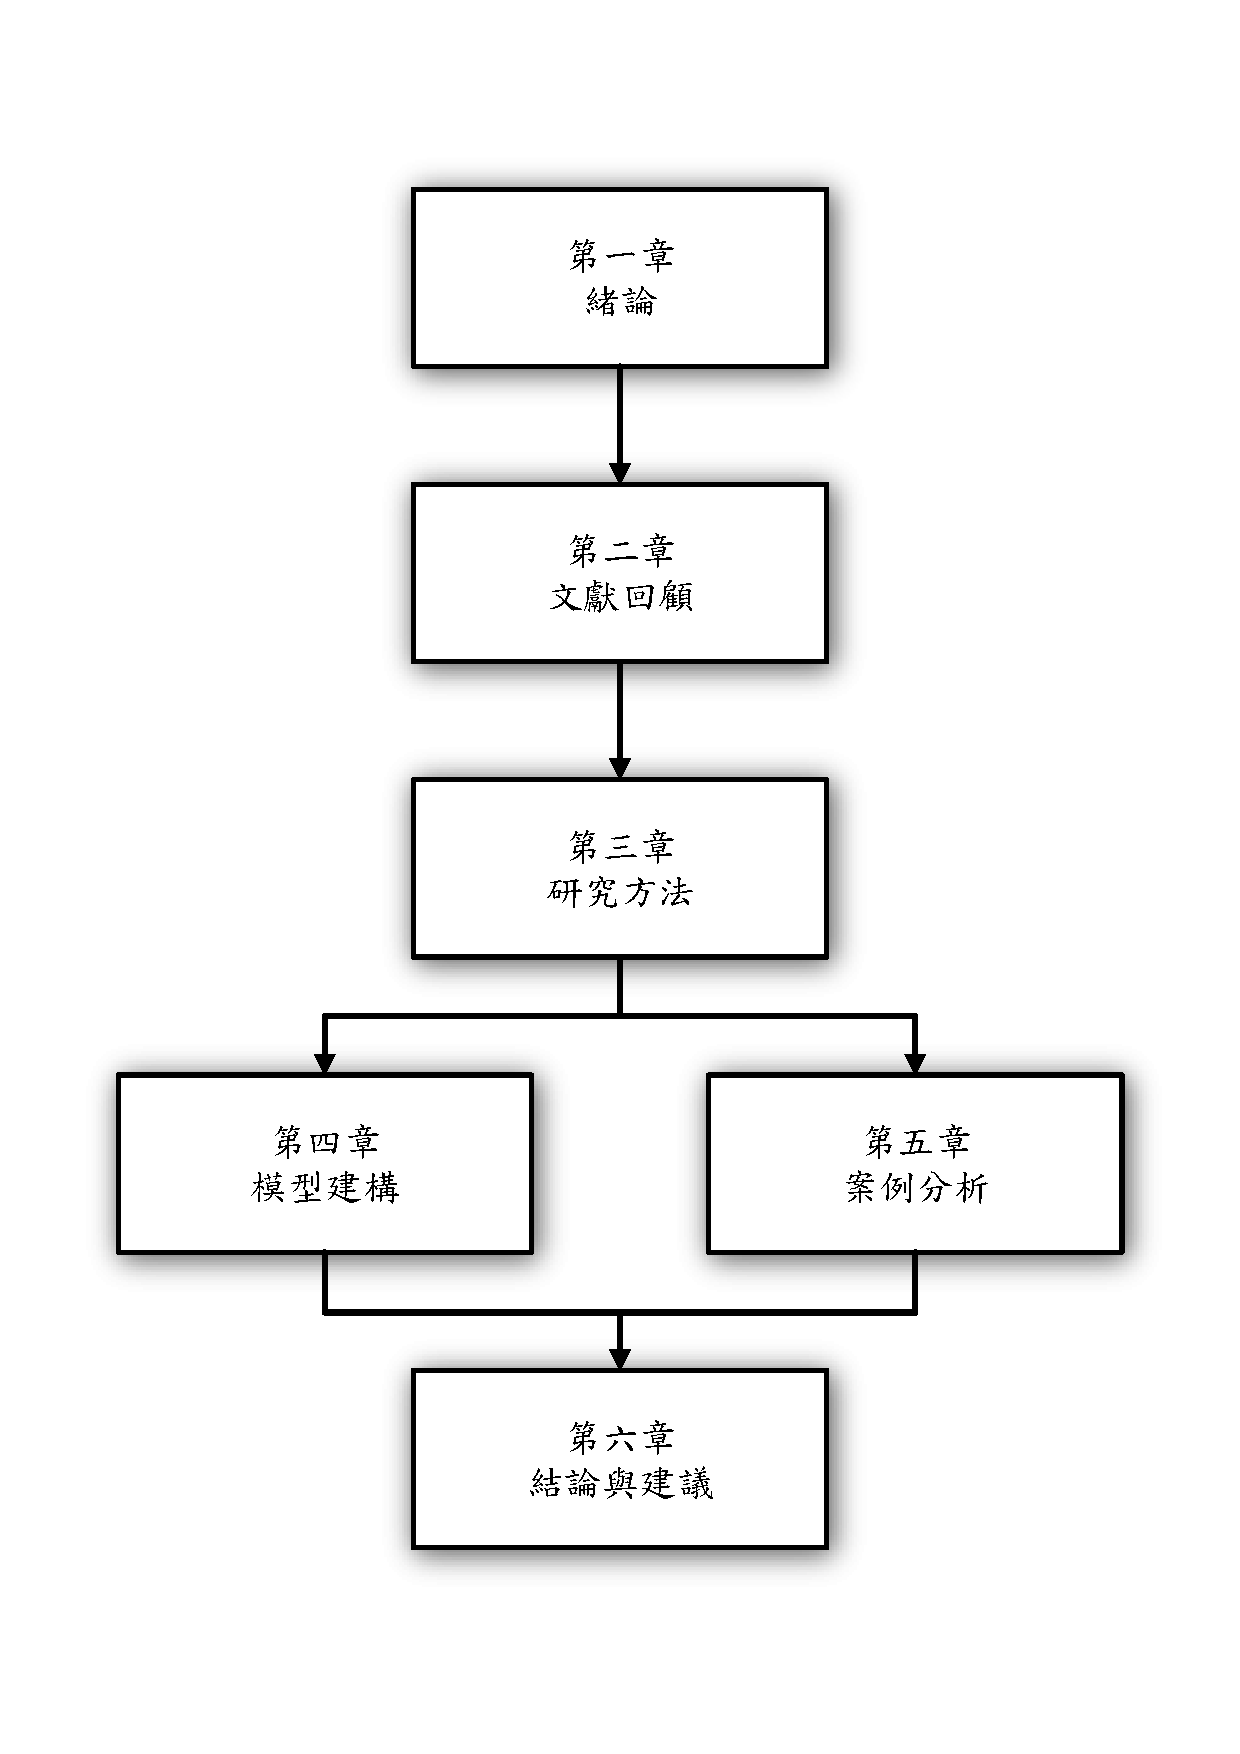
\includegraphics[width=\textwidth]{Thesis Organization}
  \caption[論文架構]{論文架構}
  \label{figure: Thesis Organization}
\end{figure}